\chapter{Examples and Constructions}

\section{Examples and Terminology}
\subsection{Example~1.1}

Suppose more generally that~$X$ is a set and~$\top{F}$ is a collection of subsets of~$X$.
There exists a (necessarily unique) topology on~$X$ whose closed sets are the sets belonging to~$\top{F}$ if and only if the following three conditions are satisfied:
\begin{itemize*}

	\item
		Both~$∅$ and~$X$ are contained in~$\top{F}$.

	\item
		$\top{F}$ is closed under intersections.

	\item
		$\top{F}$ is closed under finite unions.

\end{itemize*}
Suppose that a collection~$\top{F}'$ of subsets of~$X$ satisfies the following two conditions.
\begin{itemize*}

	\item
		$\top{F}'$ is nonempty.

	\item
		$\top{F}'$ is closed under finite unions.

	\item
		For every set~$F$ belonging to~$\top{F}'$, all subsets of~$F$ again belong to~$\top{F}'$.

\end{itemize*}
Then~$\top{F} = \top{F}' ∪ \{ X \}$ satisfies the conditions for closed sets of a topology.

It follows for both
\[
	\top{F}'_1 ≔ \{ F ⊆ X \suchthat \text{$F$ is finite} \} ∪ \{ X \}
\]
and
\[
	\top{F}'_2 ≔ \{ F ⊆ X \suchthat \text{$F$ is countable} \} ∪ \{ X \}
\]
that~$\top{F}'_1 ∪ \{ X \}$ and~$\top{F}'_2 ∪ \{ X \}$ form the closed sets for topologies on~$X$.

\subsection{Example~1.3}

We check that the collection of half-open intervals~$\basis{B} = \{ [a, b) \mid a, b ∈ ℝ, a < b \}$ is indeed a basis for a topology on~$ℝ$.

Every point~$x$ in~$ℝ$ is contained in the element~$[x, x+1)$ of~$\basis{B}$.
This shows that~$\basis{B}$ satisfies the first property of a basis.

Let~$B$ and~$C$ be two sets belonging to~$\basis{B}$ and let~$x$ be a point in the intersection~$B ∩ C$.
The sets~$B$ and~$C$ are of the form~$B = [a, b)$ and~$C = [c, d)$ for real numbers~$a$,~$b$,~$c$ and~$d$ with~$a < b$ and~$c < d$.
The intersection~$B ∩ C = [a, b) ∩ [c, d)$ is given by~$[e, f)$ for the numbers~$e = \max(a, c)$ and~$f = \min(b, d)$.
We must have~$e < f$ since~$[e, f)$ is nonempty, as~$x$ is contained in~$[e, f)$.
Therefore,~$[e, f)$ belongs to~$\basis{B}$, and we have~$x ∈ [e, f) ⊆ B ∩ C$
This shows that~$\basis{B}$ satisfies the second property of a basis.

\subsection{Example~1.4}

We check that the given collection of sets
\[
	\basis{B}
	= \{ (a, b) \suchthat a, b ∈ X, a < b \}
		∪ \{ (a, ∞) \suchthat a ∈ X \}
	  ∪ \{ (-∞, b) \suchthat b ∈ X \}
\]
is a topology for a basis on~$X$.

We first note that this statement is wrong if~$X$ is a one-element set.
We also observe that the assertion is true if~$X$ is empty (since for the empty topological space, every collection of subsets is a basis).
We will therefore assume in the following that~$X$ contains at least two different elements.

Let~$x$ be an element of~$X$.
There exist by assumption an element~$y$ of~$X$ with~$y ≠ x$, and thus either~$x < y$ or~$y < x$.
It follows that~$x$ is contained in~$(-∞, y)$ or in~$(y, ∞)$, with both of these sets belonging to~$\basis{B}$.
This shows that~$\basis{B}$ satisfies the first property of a basis.

To show that~$\basis{B}$ satisfies the second property of a basis we may extend~$\basis{B}$ to~$\basis{B}' = \basis{B} ∪ \{ X \}$, and show that~$\basis{B}$ satisfies the second property of a basis.
We also set~$X' ≔ X ∪ \{ ∞, -∞ \}$, so that
\[
	\basis{B}' = \{ (a, b) \suchthat a, b ∈ X' \} \,.
\]

Let~$B$ and~$C$ be two sets belonging to~$\basis{B}'$.
There exist elements~$a, b, c, d ∈ X'$ with~$B = (a, b)$ and~$C = (c, d)$.
The intersection~$B ∩ C$ is thus given by~$(e, f)$ with~$e = \min(a, c)$ and~$f = \max(b, d)$.
If~$x$ is a point in~$B ∩ C$ then we must have~$e < f$ whence~$B ∩ C = (e, f)$ again belongs to~$\basis{B}'$.
It follows that~$\basis{B}'$ satisfies the second property of a basis.

\subsection{Example~1.5}

We note that the proposed equation~$ℤ ∖ \{-1, 1\} = ⋃_{\text{$p$ prime}} S(p, 0)$ cannot be true with the given definition of~$S(a, b)$, since the right-hand side consists no negative integers.
Comparing with other source seems to suggest that the definition of~$S$ should use~$ℤ$ instead of~$ℕ$, so that
\[
	S(a, b) = \{ a n + b \suchthat n ∈ ℤ \} = a ℤ + b \,.
\]
In the following, we will use this definition instead.

The book isn’t quite clear on how the given topology is supposed to be defined.
\begin{itemize}

	\item
		The given formulation seems to suggest that the set
		\[
			\{ S(a, b) \suchthat a, b ∈ ℤ, a ≠ 0 \} ∪ \{ ∅ \}
		\]
		is supposed to be a topology on~$ℤ$.
		But this would be false, since the union~$S(2, 0) ∪ S(3, 0)$ would not be open again.

	\item
		One could also read the given formulation as saying that there exists \emph{some} topology on~$ℤ$ for which these sets are open.
		But this seems strange for at least two reasons:
		\begin{itemize}

			\item
				Why explicitly mention that~$∅$ is supposed to be open?
				Every topology automatically satisfies this condition.

			\item
				The existence of such a topology would be trivial, since the discrete topology would do the job.

		\end{itemize}
		The later statement that \enquote{no nonempty finite set can be open} would also not necessarily be true.
\end{itemize}

Instead, the proper claim should probably be that the set
\[
	\{ S(a, b) \suchthat a, b ∈ ℤ, a ≠ 0 \}
\]
is a basis for a topology on~$ℤ$.
We prove this claim by showing the following more general version:

\begin{proposition}
	\label{topolgies from subgroups}
	Let~$A$ be an abelian group.
	Let~$\mathcal{S}$ be a nonempty collection of subgroups of~$A$ such that for every two subgroups~$S_1$ and~$S_2$ contained in~$\mathcal{S}$, there exists a third subgroup~$T$ contained in~$\mathcal{S}$ with~$T ⊆ S_1 ∩ S_2$.
	Then the set
	\[
		\basis{B} ≔ \{ a + S \suchthat S ∈ \mathcal{S} \}
	\]
	is a basis for a topology on~$A$.
	In this topology, the sets belonging to~$\basis{B}$ are not only open but also closed.
\end{proposition}

\begin{proof}
	By assumption, there exists an element~$S$ of~$\mathcal{S}$.
	Every element~$a$ of~$A$ is then contained in the corresponding set~$a + S$ belonging to~$\basis{B}$.
	This shows that~$\basis{B}$ satisfies the first property of a basis.

	Let~$B$ and~$C$ be two elements of~$\basis{B}$ and let~$x$ be an element of~$B ∩ C$.
	There exists elements~$S_1$ and~$S_2$ of~$\basis{B}$ and elements~$a_1$ and~$a_2$ of~$A$ with~$B = a_1 + S_1$ and~$C = a_2 + S_2$.
	The sets~$a_1 + S_2$ and~$a_2 + S_2$ are cosets of~$S_1$ and~$S_2$ respectively, which contain~$x$.
	We have therefore~$a_1 + S_1 = x + S_1$ and also~$a_2 + S_2 = x + S_2$, and thus~$B = x + S_1$ and~$C = x + S_2$.
	It follows that
	\[
		B ∩ C
		=
		(x + S_1) ∩ (x + S_2)
		=
		x + (S_1 ∩ S_2) \,.
	\]
	(We note that the map~$A \to A$ given by~$a \mapsto x + a$ is bijective, and therefore preserves intersections.)
	There exists by assumption some element~$T$ of~$\mathcal{S}$ with~$T ⊆ S_1 ∩ S_2$.
	We have~$x ∈ x + T$ and~$x + T ⊆ B ∩ C$, with~$x + T$ belonging to~$\basis{B}$.
	This shows that~$\basis{B}$ satisfies the second property of a basis.

	Let~$B$ be a set belonging to~$\basis{B}$.
	This set is of the form~$B = a + S$ for some~$a ∈ A$ and a subgroup~$S$ belonging to~$\mathcal{S}$.
	The complement of~$B$ is the union of all other cosets of~$S$, all of which also belong to~$\basis{B}$ and are therefore open.
	The complement of~$B$ is therefore open, whence~$B$ is closed.
\end{proof}

The above \lcnamecref{topolgies from subgroups} has the following special cases:
\begin{itemize*}

	\item
		For every integral domain~$R$ we can choose~$\mathcal{S}$ as the set of nonzero ideals of~$R$: for every two ideals~$I$ and~$J$ of~$R$, the product~$IJ$ is again nonzero.
		(The intersection~$I ∩ J$ is therefore also nonzero, as it contains~$IJ$.)

	\item
		For every ring~$R$ and every ideal~$I$ we can choose~$\mathcal{S}$ is the set of ideals~$I^k$ with~$k ≥ 0$.
		(The resulting topology on~$R$ is the~$I$\nobreakdash-adic topology.)

\end{itemize*}

We have thus shown that there exists a topology on~$ℤ$ with basis given by~$\{ S(a, b) \suchthat a, b ∈ ℤ, a ≠ 0 \}$, and each of these basis open sets is also closed.
Every basis open set is infinite, whence every nonempty open set is infinite.
The set~$ℤ ∖ \{-1, 1\}$ is therefore not closed.
But the set~$S(p, 0)$ is closed for each prime~$p$, and the union of finitely many closed sets is again closed.
We thus find from the equality~$ℤ ∖ \{-1, 1\} = ⋃_{\text{$p$ prime}} S(p, 0)$ that there are infinitely many primes.

\subsection{Example~1.6}

We will verify in \nameref{exercise 1.3} that the Zariski topology is indeed a topology.

\subsection{Example~1.8}

That~$\ell_∞$ is not homeomorphic to~$ℓ_p$ for~$1 ≤ p < ∞$ will be shown in \nameref{exercise 1.6}.

\subsection{Example~1.12}

We have for every two points~$y$ and~$z$ in~$X$ the (in)equalities
\[
	f y
	=
	d(x, y)
	≤
	d(x, z) + d(z, y)
	=
	f z + d(y, z) \,,
\]
and therefore the inequality
\[
	f y - f z ≤ d(y, z) \,.
\]
By swapping the roles of~$y$ and~$z$ we get also the inequality
\[
	f z - f y ≤ d(z, y) = d(y, z) \,.
\]
We can combine both of these inequalities into the single inequality
\[
	\abs{f y - f z} ≤ d(y, z) \,.
\]
This inequality tells us that the function~$f$ is Lipschitz continuous, and therefore continuous.


\section{The Subspace Topology}
\subsection{Definition 1.1}

We check that~$\top{T}_Y$ is indeed a topology on~$Y$.

We have~$∅ ∈ \top{T}_X$ and~$∅ ∩ Y = ∅$, and therefore~$∅ ∈ \top{T}_Y$.
We similarly have~$X ∈ \top{T}_X$ and~$X ∩ Y = Y$, and therefore~$Y ∈ \top{T}_Y$.

Let~$(V_α)_{α ∈ A}$ be a family of elements of~$\top{T}_Y$.
For every index~$α ∈ A$ there exists an element~$U_α$ of~$\top{T}_X$ with~$V_α = U_α ∩ Y$.
The union~$U ≔ ⋃_{α ∈ A} U_α$ is again an element of~$\top{T}_X$, for which we have
\[
	U ∩ Y
	=
	\Biggl( ⋃_{α ∈ A} U_α \Biggr) ∩ Y
	=
	⋃_{α ∈ A} {} (U_α ∩ Y)
	=
	⋃_{α ∈ A} V_α \,.
\]
This shows that the union~$⋃_{α ∈ A} V_α$ is again contained in~$\top{T}_Y$.

Let~$V_1, \dotsc, V_n$ be elements of~$\top{T}_Y$.
There exists for every index~$i = 1, \dotsc, n$ an element~$U_i$ of~$\top{T}_X$ with~$V_i = U_i ∩ Y$.
The intersection~$U ≔ U_1 ∩ \dotsb ∩ U_n$ is again an element of~$\top{T}_X$, and we have
\[
	U ∩ Y
	=
	(U_1 ∩ \dotsb ∩ U_n) ∩ Y
	=
	(U_1 ∩ Y) ∩ \dotsb ∩ (U_n ∩ Y)
	=
	V_1 ∩ \dotsb ∩ V_n \,.
\]
This shows that the intersection~$V_1 ∩ \dotsb ∩ V_n$ is again an element of~$\top{T}_Y$.

\subsection{Coarsest and Finest Topologies for Continuity}

We make the following general observations:

\begin{proposition}
	\label{pullback and pushforward of topologies}
	Let~$f \colon X \to Y$ be a function between sets.
	\begin{enumerate}

		\item
			For every topology~$\top{T}_X$ on~$X$ there exists a finest topology~$f_* \top{T}_X$ on~$Y$ such that~$f$ is continuous with respect to~$\top{T}_X$ and~$f_* \top{T}_X$, and this topology is given by
			\[
				f_* \top{T}_X = \{ U ⊆ Y \suchthat f^{-1} U ∈ \top{T}_X \} \,.
			\]

		\item
			For every topology~$\top{T}_Y$ on~$Y$ there exists a coarsest topology~$f^* \top{T}_Y$ on~$X$ such that~$f$ is continuous with respect to~$f^* \top{T}_Y$ and~$\top{T}_Y$, and this topology is given by
			\[
				f^* \top{T}_Y = \{ f^{-1} U \suchthat U ∈ \top{T}_Y \} \,.
			\]

		\item
			For every topology~$\top{T}_X$ on~$X$ and every topology~$\top{T}_Y$ on~$Y$ we have the equivalences
			\[
				f^* \top{T}_Y ⊆ \top{T}_X
				\iff
				\text{$\textstyle f \colon (X, \top{T}_X) \to (Y, \top{T}_Y)$ is continuous}
				\iff
				\top{T}_Y ⊆ f_* \top{T}_X \,.
			\]

	\end{enumerate}
\end{proposition}

\begin{proof}
	\leavevmode
	\begin{enumerate}

		\item
			Is suffices to show that the given set~$f_* \top{T}_X$ is a topology on~$Y$.

			We have~$∅ ∈ f_* \top{T}_X$ because~$f^{-1} ∅ = ∅ ∈ \top{T}_X$, and similarly~$Y ∈ f_* \top{T}_X$ because~$f^{-1} Y = X ∈ \top{T}_X$.

			Let~$(U_α)_{α ∈ A}$ be a family of sets belonging to~$f_* \top{T}_X$.
			This means that~$f^{-1} U_α$ belongs to~$\top{T}_X$ for every index~$α$.
			It follows that
			\[
				f^{-1} ⋃_{α ∈ A} U_α
				=
				⋃_{α ∈ A} f^{-1} U_α
				\in
				\top{T}_X
			\]
			since~$\top{T}_X$ is a topology.
			This shows that the union~$⋃_{α ∈ A} U_α$ again belongs to~$f_* \top{T}_X$.

			Let~$U_1, \dotsc, U_n$ be finitely many subsets of~$Y$ belonging to~$f_* \top{T}_X$.
			This means that~$f^{-1} U_i$ belongs to~$\top{T}_X$ for every index~$i$.
			It follows that
			\[
				f^{-1} (U_1 ∩ \dotsb ∩ U_n)
				=
				f^{-1} U_1 ∩ \dotsb ∩ f^{-1} U_n
				\in
				\top{T}_X
			\]
			since~$\top{T}_X$ is a topology.
			This shows that the intersection~$U_1 ∩ \dotsb ∩ U_n$ again belongs to~$f_* \top{T}_X$.

		\item
			It suffices to show that~$f^* \top{T}_Y$ is a topology on~$X$.
			We have~$∅ = f^{-1} ∅ ∈ f^* \top{T}_X$ because~$∅$ belongs to~$\top{T}_Y$.
			We have similarly~$X = f^{-1} Y ∈ f^* \top{T}_X$ because~$Y$ belongs to~$\top{T}_Y$.

			Let~$(V_α)_{α ∈ A}$ be a family of sets belonging to~$f^* \top{T}_Y$.
			This means that for every index~$α$ there exists a set~$U_α$ belonging to~$\top{T}_Y$ with~$V_α = f^{-1} U_α$.
			The union~$⋃_{α ∈ A} U_α$ again belongs to~$\top{T}_Y$ because~$\top{T}_Y$ is a topology.
			It follows that the union
			\[
				⋃_{α ∈ A} V_α
				=
				⋃_{α ∈ A} f^{-1} U_α
				=
				f^{-1} ⋃_{α ∈ A} U_α
			\]
			again belongs to~$f^* \top{T}_Y$.

			Let~$V_1, \dotsc, V_n$ be finitely many sets belonging to~$f^* \top{T}_X$.
			This means that for every index~$i$ there exists a set~$U_i$ belonging to~$\top{T}_Y$ with~$V_i = f^{-1} U_i$.
			The intersection~$U_1 ∩ \dotsb ∩ U_n$ again belongs to~$\top{T}_Y$ because~$\top{T}_Y$ is a topology.
			It follows that the intersection
			\[
				V_1 ∩ \dotsb ∩ V_n
				=
				f^{-1} U_1 ∩ \dotsb ∩ f^{-1} U_n
				=
				f^{-1} (U_1 ∩ \dotsb ∩ U_n)
			\]
			again belongs to~$f^* \top{T}_Y$.

		\item
			The map~$f$ is continuous with respect to~$\top{T}_X$ and~$\top{T}_Y$ if and only if for every set~$U$ belonging to~$\top{T}_Y$ its preimage~$f^{-1} U$ belongs to~$\top{T}_Y$.
			This condition can be expressed as~$f^* \top{T}_Y ⊆ \top{T}_X$, but also as~$\top{T}_Y ⊆ f^* \top{T}_X$.
		\qedhere

	\end{enumerate}
\end{proof}

\begin{proposition}
	Let~$f \colon X \to Z$ and~$g \colon Y \to Z$ be two composable functions between sets.
	\begin{enumerate}[resume]

		\item
			For every topology~$\top{T}_X$ on~$X$, we have~$g_* f_* \top{T}_X = (gf)_* \top{T}_X$.

		\item
			For every topology~$\top{T}_Z$ on~$Z$, we have~$f^* g^* \top{T}_Z = (gf)^* \top{T}_Z$.

	\end{enumerate}
\end{proposition}

\begin{proof}
	\leavevmode
	\begin{enumerate}

		\item
			For every subset~$W$ of~$Z$ we have the chain of equivalences
			\begin{align*}
				W ∈ g_* f_* \top{T}_X
				&\iff
				g^{-1} W ∈ f_* \top{T}_X \\
				&\iff
				f^{-1} g^{-1} W ∈ \top{T}_X \\
				&\iff
				(g f)^{-1} W ∈ \top{T}_X \\
				&\iff
				W ∈ (g f)_* \top{T}_X \,.
			\end{align*}
			This shows that indeed~$g_* f_* \top{T}_X = (g f)_* \top{T}_X$.

		\item
			We have the chain of equalities
			\begin{align*}
				f^* g^* \top{T}_Z
				&=
				\{ f^{-1} V \suchthat V ∈ g^* \top{T}_Z \} \\
				&=
				\{ f^{-1} g^{-1} U \suchthat U ∈ \top{T}_Z \} \\
				&=
				\{ (g f)^{-1} U \suchthat U ∈ \top{T}_Z \} \\
				&=
				(g f)^* \top{T}_Z \,,
			\end{align*}
			showing the assertion.
		\qedhere

	\end{enumerate}
\end{proof}

\begin{corollary}
	Let~$f \colon X \to Y$ be a function between sets.
	\begin{enumerate}

		\item
			Let~$\top{T}_X$ be a topology on~$X$.
			Let~$Z$ be a topological space and let~$g$ be a map from~$Y$ to~$Z$.
			The map~$g$ is continuous from~$(Y, f_* \top{T}_X)$ to~$Z$ if and only if the composite~$g f$ is continuous from~$(X, \top{T}_X)$ to~$Z$.

		\item
			Let~$\top{T}_Y$ be a topology on~$Y$.
			Let~$Z$ be a topological space and let~$h$ be a map from~$Z$ to~$X$.
			The map~$h$ is continuous from~$Z$ to~$(X, f^* \top{T}_Y)$ if and only if the composite~$f h$ is continuous from~$Z$ to~$(Y, \top{T}_Y)$.

	\end{enumerate}
\end{corollary}

\begin{proof}
	In both cases let~$\top{T}_Z$ denote the topology on~$Z$.
	\begin{enumerate}

		\item
			We observe the chain of equivalences
			\begin{align*}
				{}&
				\text{$g$ is continuous from~$(Y, f_* \top{T}_X)$ to~$Z$} \\
				\iff{}&
				g^* \top{T}_Z ⊆ f_* \top{T}_X \\
				\iff{}&
				f^* g^* \top{T}_Z ⊆ \top{T}_X \\
				\iff{}&
				(g f)^* \top{T}_Z ⊆ \top{T}_X \\
				\iff{}&
				\text{$g f$ is continuous from~$(X, \top{T}_X)$ to~$Z$} \,.
			\end{align*}

		\item
			We observe similarly the chain of equivalences
			\begin{align*}
				{}&
				\text{$h$ is continuous from~$Z$ to~$(X, f^* \top{T}_Y)$} \\
				\iff{}&
				f^* \top{T}_Y ⊆ h_* \top{T}_Z \\
				\iff{}&
				h^* f^* \top{T}_Y ⊆ \top{T}_Z \\
				\iff{}&
				(f h)^* \top{T}_Y ⊆ \top{T}_Z \\
				\iff{}&
				\text{$f h$ is continuous from~$Z$ to~$(Y, \top{T}_Y)$} \,.
			\end{align*}
			This shows the assertion.
		\qedhere

	\end{enumerate}
\end{proof}

\subsection{Example~1.15}

The statement about the subspace topology on~$ℝ$ is not correct:
the given sets~$ℚ ∩ (a, b)$ are only a basis for the subspace topology on~$ℚ$.
In other words, every open subset of~$ℚ$ is a union of sets of the form~$ℚ ∩ (a, b)$ with~$a < b$.


\section{The Quotient Topology}
\subsection{Better Definition of the Quotient Topology}

The author thinks that the \enquote{word of caution} may be slightly misleading.

The set~$\mathscr{T}$ of topologies on~$X$ forms a partially ordered set with respect to subset inclusion~$⊆$.
For every family~$(\top{T}_α)_{α ∈ A}$ of topologies on~$X$, the intersection~$⋂_{α ∈ A} \top{T}_α$ is again a topology on~$X$;
this is the finest topology on~$X$ that is coarser than all~$\top{T}_α$.
Equivalently, every subset of~$\mathscr{T}$ admits an infimum.

Therefore,~$\mathscr{T}$ is a complete lattice.

But this entails that every subset of~$\mathscr{T}$ also admits a supremum.
In other words, for every family~$(\top{T}_α)_{α ∈ A}$ of topologies on~$X$, there exists a coarsest topology that is finer than all~$\top{T}_α$.
This topology is more explicitly given by the topology generated by the union~$⋃_{α ∈ A} \top{T}_α$.

Suppose now that~$P$ is some property of topologies on~$X$.
This is, for every topology~$\top{T}$ on~$X$, the property~$P(\top{T})$ is either true or false.
We can then consider the set~$\mathscr{T}_P$ of all topologies on~$X$ that satisfy~$P$:
\[
	\mathscr{T}_P = \{ \top{T} ∈ \mathscr{T} \suchthat P(\top{T}) \} \,.
\]
The set~$\mathscr{T}_P$ admits both a supremum~$\top{T}_{\sup}$ and an infimum~$\smash{\top{T}}_{\inf}$ in~$\mathscr{T}$.

There exists a finest topology on~$X$ satisfying~$P$ if and only if~$\smash{\top{T}}_{\sup}$ is contained in~$\mathscr{T}_P$, and there exists a coarsest topology on~$X$ satisfying~$P$ if and only if~$\smash{\top{T}}_{\inf}$ is contained in~$\mathscr{T}_P$.

We see that, at least from a certain theoretical perspective, the issues of having a finest topology satisfying~$P$ and having a coarsest topology satisfying~$P$ are equivalently problematic.

We fix some notation for further use.

\begin{definition}
	\label{notation for infima and suprema of topologies}
	Let~$X$ be a set and let~$\mathscr{T}$ be a collection of topologies on~$X$.
	\begin{enumerate}

		\item
			The coarsest topology on~$X$ that is finer than every topology contained in~$\mathscr{T}$ is denoted by~$⋀ \mathscr{T}$.

		\item
			The finest topology on~$X$ that is coarser than every topology contained in~$\mathscr{T}$ is denoted by~$⋁ \mathscr{T}$.

	\end{enumerate}
\end{definition}

\subsection{Universal Property of the Quotient Topology}

Using the notation introduced in \cref{pullback and pushforward of topologies}, the quotient topology on~$S$ is precisely the topology~$π_* \top{T}_X$, where~$\top{T}_X$ is the topology of~$X$.
The desired universal property therefore follows from \cref{universal properties for pullback and pushforward of topologies}.

\subsection{Example~1.18}

We will prove that the third space is indeed~$ℝℙ^2$.
We will proceed in four steps:
\begin{enumerate*}

	\item
		We first replace the unit square~$\int^2$ by the unit disk~$\disk^2$.

	\item
		Next we identify the disk~$\disk^2$ with the upper hemisphere~$H$ of the unit sphere~$\sphere^2$.

	\item
		We show that the inclusion map from~$H$ to~$\sphere^2$ induces a homeomorphism from~$H / {∼}$ to~$\sphere^2 / {∼}$, where the equivalence relation~$∼$ identifies antipodal points.

	\item
		We construct a homeomorphism between~$\sphere^2 / {∼}$ and~$ℝℙ^2$.

\end{enumerate*}
At the heart of our argumentation lies the following observations:

\begin{lemma}
	\label{functoriality of the quotient}
	Let~$X$ and~$Y$ be two topological spaces together with equivalence relations on them.
	Let~$f \colon X \to Y$ be a continuous map with
	\begin{equation}
		\label{map is compatible with equivalence relation}
		x_1 ∼ x_2 \implies f x_1 ∼ f x_2
	\end{equation}
	for all~$x_1, x_2 ∈ X$.
	Then~$f$ indues a continuous map
	\[
		X / {∼} \to Y / {∼} \,,
		\quad
		\class{x} \mapsto \class{f x} \,.
	\]
	In terms of a commutative diagram:
	\[
		\begin{tikzcd}
			X
			\arrow{r}[above]{f}
			\arrow{d}
			&
			Y
			\arrow{d}
			\\
			X / {∼}
			\arrow[dashed]{r}
			&
			Y / {∼}
		\end{tikzcd}
	\]
\end{lemma}

\begin{proof}
	Let~$π_X \colon X \to X / {∼}$ and~$π_Y \colon Y \to Y / {∼}$ be the canonical quotient maps.
	The map~$π_Y f \colon X \to Y / {∼}$ is continuous and induces a well-defined map~$g \colon X / {∼} \to  Y / {∼}$ with $g \class{x} = \class{fx}$.
	It follows from the universal property of the quotient~$X / {∼}$ that~$g$ is continuous.
\end{proof}

\begin{proposition}
	\label{induced homeomorphism between quotients}
	Let~$X$ and~$Y$ be two homeomorphic topological spaces and suppose we are given equivalence relations on~$X$ and~$Y$.
	Suppose that there exists a homeomorphism~$φ \colon X \to Y$ with
	\[
		x_1 ∼ x_2 \iff φ x_1 ∼ φ x_2
	\]
	for all~$x_1, x_2 ∈ X$.
	The homeomorphism~$φ$ induces a homeomorphism
	\[
		X / {∼} \to Y / {∼} \,,
		\quad
		\class{x} \mapsto \class{φ x} \,.
	\]
	Consequently,~$X / {∼}$ and~$Y / {∼}$ are again homeomorphic.
\end{proposition}

\begin{proof}
	We find from \cref{functoriality of the quotient} that the continuous maps~$φ$ and~$φ^{-1}$ induce continuous maps
	\[
		ψ \colon X / {∼} \to Y / {∼} \,, \quad \class{x} \mapsto \class{φ x}
	\]
	and
	\[
		ψ' \colon Y / {∼} \to X / {∼} \,, \quad \class{y} \mapsto \class{φ^{-1} y} \,.
	\]
	The maps~$ψ$ and~$ψ'$ are again mutually inverse.
	Therefore,~$ψ$ is a homeomorphism from~$X / {∼}$ to~$Y / {∼}$ with inverse~$ψ'$.
\end{proof}

We will also use the dual observation regarding subspaces.

\begin{lemma}
	\label{restriction of continuous maps to subspaces}
	Let~$X$ and~$Y$ be two topological spaces, let~$S ⊆ X$ and~$T ⊆ Y$ be subspaces and let~$f \colon X \to Y$ be a continuous map with~$f X ⊆ Y$.
	Then~$f$ restricts to a continuous map from~$S$ to~$T$.
	In terms of a commutative diagram:
	\[
		\begin{tikzcd}
			X
			\arrow{r}[above]{f}
			&
			Y
			\\
			S
			\arrow{u}
			\arrow[dashed]{r}
			&
			T
			\arrow{u}
		\end{tikzcd}
	\]
\end{lemma}

\begin{proof}
	Let~$i \colon S \to X$ and~$j \colon T \to Y$ be the inclusion maps.
	It follows from the condition~$f S ⊆ T$ that~$f$ restricts to a map~$g$ from~$S$ to~$T$.
	The composite~$j g = f i$ is continuous, so it follows from the universal property of the subspace topology on~$T$ that~$g$ is continuous.
\end{proof}

\begin{proposition}
	\label{restriction of homeomorphism to subspaces}
	Let~$φ \colon X \to Y$ be a homeomorphism.
	Let~$S ⊆ X$ and~$T ⊆ Y$ be subspaces with~$φ S = T$.
	Then~$φ$ restricts to a homeomorphism from~$S$ to~$T$.
\end{proposition}

\begin{proof}
	It follows from the bijectivity of~$φ$ and the condition~$φ S = T$ that also~$φ^{-1} T = S$.
	It follows from \cref{restriction of homeomorphism to subspaces} that the two homeomorphisms~$φ$ and~$φ^{-1}$ restricts to continuous maps~$ψ \colon S \to T$ and~$ψ' \colon T \to S$.
	These two maps are again mutually inverse.
	Therefore,~$ψ$ is a homeomorphism with inverse~$ψ'$.
\end{proof}

We will also use the following glueing principle.

\begin{lemma}
	\label{closed subsets in the subset topology}
	Let~$X$ be a topological space and let~$Y$ be a subspace of~$X$.
	Every closed subset of~$Y$ is of the form~$C ∩ Y$ for a closed subset of~$X$.
\end{lemma}

\begin{proof}
	Let~$C'$ be a closed subset of~$Y$.
	This means that the complement~$Y ∖ C'$ is open in~$Y$, whence there exists an open subset~$U$ of~$X$ with~$Y ∖ C' = U ∩ Y$.
	The set~$C ≔ Y ∖ U$ is closed in~$X$ with
	\[
		C' = Y ∖ (Y ∖ C') = Y ∖ (U ∩ Y) = (X ∖ U) ∩ Y \,,
	\]
	as desired.
\end{proof}

\begin{lemma}
	\label{closed subsets of closed subspaces are closed}
	Let~$X$ be a topological space and let~$Y$ be a closed subspace of~$X$.
	Let~$C$ be a closed subset of~$Y$.
	Then~$C$ is also closed in~$X$.
\end{lemma}

\begin{proof}
	There exists by \cref{closed subsets in the subset topology} a closed subset~$C'$ of~$X$ with~$C = C' ∩ Y$.
	Both~$C'$ and~$Y$ are closed in~$X$, so their intersection is again closed in~$X$.
\end{proof}

\begin{proposition}
	\label{glueing continuous functions on closed subspaces}
	Let~$X$ and~$Y$ be two topological spaces an let~$f \colon X \to Y$ be a map.
	Suppose that~$X = A ∪ B$ for two closed subsets~$A$ and~$B$ of~$X$ and that the restrictions~$\restrict{f}{A}$ and~$\restrict{f}{B}$ are continuous (with respect to the subspace topologies).
	Then~$f$ is continuous.
\end{proposition}

\begin{proof}
	We need to show that for every closed subset~$C$ of~$Y$ its preimage~$f^{-1} C$ is closed in~$X$.
	We have the equality~$f^{-1} C = (\restrict{f}{A})^{-1} C ∪ (\restrict{f}{B})^{-1} C$, whence it suffices to show that both~$(\restrict{f}{A})^{-1} C$ and~$(\restrict{f}{B})^{-1} C$ are closed in~$X$.
	But~$A$ and~$B$ are closed in~$C$, so by \cref{closed subsets of closed subspaces are closed} it suffices to show that~$(\restrict{f}{A})^{-1} C$ is closed in~$A$ and~$(\restrict{f}{B})^{-1} C$ is closed in~$B$.
	This holds because both~$\restrict{f}{A}$ and~$\restrict{f}{B}$ are continuous.
\end{proof}



\subsubsection{Zeroth Step}

To make the next step easier, we replace the unit square~$\int^2 = [0, 1] × [0, 1]$ with the square
\[
	S ≔ [-1, 1] × [-1, 1]
\]
that is centered around the origin.
More explicitly, we consider the map
\[
	φ \colon \int^2 \to S \,, \quad 2 x - (1, 1) \,.
\]
The map~$φ$ is continuous and bijective, and its inverse
\[
	φ^{-1} \colon S \to \int^2 \,, \quad x \mapsto \frac{1}{2} (x + (1, 1))
\]
is again continuous.
Therefore,~$φ$ is a homeomorphism.

The equivalence relation on~$\int^2$ described in the book identifies antipodal points on the boundary of~$\int^2$.
It follows that the corresponding equivalence relation on~$S$ also identifies antipodal points on the boundary (because of the specific form that~$φ$ has).
More explicitly, we have $(x, 1) ∼ (-x, -1)$ and~$(1, y) ∼ (-1, -y)$ for all~$x, y ∈ [-1, 1]$.



\subsubsection{First Step}

For the first step we construct a homeomorphism between the square~$S$ and the unit disk
\[
	\disk^2 = \{ x ∈ ℝ^2 \suchthat \norm{x} ≤ 1 \} \,.
\]
We observe that we can rewrite the square~$S$ as
\[
	S = \{ x ∈ ℝ^2 \suchthat \norm{ x }_∞ ≤ 1 \} \,.
\]
We know that the norms~$\norm{ \phdot }$ and~$\norm{ \phdot }_∞$ induce the same topology on~$ℝ^2$.
This motivates the following observation:

\begin{proposition}
	Let~$V$ be a vector space and let~$\norm{\phdot}_1$ and~$\norm{\phdot}_2$ be two norms on~$V$ that induce the same topology.
	The rescaling map
	\[
		ρ
		\colon
		V
		\to
		V \,,
		\quad
		x
		\mapsto
		\begin{cases*}
			\dfrac{\norm{x}_1}{\norm{x}_2} x & if~$x ≠ 0$, \\[0.2em]
			0                              & if~$x = 0$,
		\end{cases*}
		\]
		is a homeomorphism.
\end{proposition}

\begin{proof}
	We start by showing that~$ρ$ is continuous.
	We use that continuity is a pointwise property:
	we show that for every point~$x$ in~$V$ the map~$ρ$ is continuous at~$x$.

	If~$x ≠ 0$, then there exists an open neighbourhood~$U$ of~$x$ that doesn’t contain the origin.
	The map~$ρ$ is given by~$ρ y = \norm{y}_1 / \norm{y}_2 ⋅ y$ for every~$y ∈ U$.
	Both~$\norm{\phdot}_1$ and~$\norm{\phdot}_2$ are continuous on~$V$, so we find that~$ρ$ is continuous on~$U$.
	This entails that~$ρ$ is continuous at~$x$.

	Suppose now that~$x = 0$.
	We will use that we are working with a normed vector spaces, whence continuity is equivalent to sequential continuity.
	So let~$(x_n)_n$ be a sequence in~$V$ with~$x_n \to 0$.
	Then
	\[
		\norm{ρ x}_2 = \norm{x}_1 \to 0
	\]
	as~$n \to ∞$, and therefore~$ρ x_n \to 0 = ρ(x)$.
	This shows that~$ρ$ is sequentially continuous at~$x$, and therefore continuous at~$x$.

	We have thus shown that~$ρ$ is continuous.
	By switching the roles of~$\norm{\phdot}_1$ and~$\norm{\phdot}_2$ we get another rescaling map~$ρ'$, which is again continuous.
	The two rescaling maps~$ρ$ and~$ρ'$ are mutually inverse, whence~$ρ$ is a homeomorphism with inverse~$ρ'$.
\end{proof}

It follows that the rescaling map
\[
	ρ
	\colon
	ℝ^2
	\to
	ℝ^2 \,,
	\quad
	x
	\mapsto
	\begin{cases*}
		\dfrac{\norm{x}_∞}{\norm{x}} x & if~$x ≠ 0$, \\[0.2em]
		0                              & if~$x = 0$,
	\end{cases*}
\]
is a homeomorphism.
We have~$\norm{ρ(x)} = \norm{x}_∞$ for every point~$x$ in~$ℝ^2$, and consequently~$ρ \disk^2 = S$.
The homeomorphism~$ρ$ therefore restricts to a homeomorphism from~$\disk^2$ to~$S$ by \cref{restriction of homeomorphism to subspaces}.

The boundary of~$\disk^2$ is mapped onto the boundary of~$S$, with antipodal points mapped to antipodal points.
The equivalence relation on~$\disk^2$ corresponding to the equivalence relation on~$S$ therefore also identifies antipodal boundary points.
More explicitly, we have~$x ∼ -x$ for every~$x ∈ \disk^2$ with~$\norm{x} = 1$, i.e., for every~$x ∈ \sphere^1$.



\subsubsection{Second Step}

We consider now the sphere~$\sphere^2 = \{ x ∈ ℝ^3 \suchthat \norm{x} = 1 \}$, and its upper hemisphere
\[
	H^+ = \{ (x, y, z) ∈ \sphere^2 \suchthat z ≥ 0 \} \,.
\]
We can flatten~$H$ down onto the disk via the continuous map
\[
	φ \colon H^+ \to \disk^2 \,, \quad (x, y, z) \mapsto (x, y) \,.
\]
We can conversely dent the disk into the upper hemisphere via the continuous map
\[
	\disk^2 \to H^+ \,, \quad (x, y) \mapsto (x, y, \sqrt{1 - x^2 - y^2}) \,.
\]
These two maps are mutually inverse, whence~$φ$ is a homeomorphism.

The homeomorphism~$φ$ maps the boundary of~$\disk^2$ onto the boundary
\[
	∂ H^+ = \{ (x, y, 0) \suchthat (x, y) ∈ \sphere^1 \} \,,
\]
and maps antipodal points to antipodal points.
The equivalence relation on the hemisphere~$H^+$ corresponding to the equivalence relation of~$\disk^2$ is therefore once again given by identifying antipodal boundary points.
More explicitly, we have~$(x, y, 0) ∼ (-x, -y, 0)$ for every~$(x, y) ∈ \sphere^1$.



\subsubsection{Third Step}

We consider the equivalence relation~$∼$ on~$\sphere^2$ given by~$x ∼ -x$ for every~$x ∈ \sphere^2$.
We find from \cref{induced homeomorphism between quotients} that the map~$i$ induces a continuous bijection
\[
	φ
	\colon
	H^+ / {∼} \to \sphere^2 / {∼} \,,
	\quad
	\class{x} \mapsto \class{x} \,.
\]

To construct the inverse of~$φ$ we consider the canonical quotient map
\[
	ψ^+ \colon H^+ \to H^+ / {∼} \,, \quad x \mapsto \class{x} \,,
\]
as well as the lower hemisphere
\[
	H^- = \{ (x, y, z) ∈ \sphere^2 \suchthat z ≤ 0 \}
\]
and the map
\[
	ψ^- \colon H^- \to H^+ / {∼} \,, \quad x \mapsto \class{-x} \,.
\]
The quotient map~$ψ^+$ is continuous, and the map~$ψ^-$ is also continuous since it is the composite of~$ψ^+$ and the continuous map~$x \mapsto -x$ from~$H^-$ to~$H^+$.
Both~$H^+$ and~$H^-$ are closed subsets of~$\sphere^2$, and~$ψ^+$ and~$ψ^-$ agree on the intersection~$H^+ ∩ H^- = ∂ H^+$ (because~$ψ^+$ agrees on antipodal poits of~$∂ H^+$).
It follows from \cref{glueing continuous functions on closed subspaces} that the two continuous maps~$ψ^+$ and~$ψ^-$ combine into a single continuous map
\[
	ψ'
	\colon
	\sphere^2 \to H^+ / {∼} \,,
	\quad
	(x, y, z)
	\mapsto
	\begin{cases*}
		\class{(x, y, z)}    & if~$z ≥ 0$, \\
		\class{(-x, -y, -z)} & if~$z ≤ 0$.
	\end{cases*}
\]
This map identifies antipodal points and therefore induces a well-defined map
\[
	ψ \colon \sphere^2 / {∼} \to H^+ / {∼} \,, \quad \class{x} \mapsto ψ' x \,.
\]
This map is again continuous by the universal property of the quotient~$\sphere^2 / {∼}$.

The two maps~$φ$ and~$ψ$ are mutually inverse, so~$φ$ is an isomorphism with inverse~$ψ$.



\subsubsection{Fourth Step}

It follows from \cref{functoriality of the quotient} that the inclusion map from~$\sphere^2$ to~$ℝ^3 ∖ \{0\}$ induces a continuous map
\[
	φ \colon \sphere^2 / {∼} \to ℝℙ^2 \,, \quad \class{x} \mapsto \class{x} \,.
\]
We can consider on the other hand the continuous map
\[
	ψ' \colon ℝ^3 ∖ \{0\} \to \sphere^2 \,, \quad x \mapsto \frac{x}{\norm{x}} \,.
\]
It follows from \cref{functoriality of the quotient} that the map~$ψ'$ induces a continuous map
\[
	ψ
	\colon
	ℝℙ^2 \to \sphere^2 / {∼} \,,
	\quad
	\class{x} \mapsto \class[\bigg]{ \frac{x}{\norm{x}} } \,.
\]
The two maps~$φ$ and~$ψ$ are mutually inverse.
Therefore,~$φ$ is a homeomorphism.


\section{The Product Topology}
\subsection{Better Definition of the Product Topology}

We will prove the universal property of the product topology as part of \nameref{exercise 1.8}.

\subsection{Universal Property for the Product Topology}

Let more generally~$X$ be a topological space and let~$(X_α)_{α ∈ A}$ be a family of topological spaces together with continuous maps~$π_α \colon X \to X_α$.
Suppose that the topology on~$X$ is the coarsest topology for which all the maps~$π_α$ are continuous.
We claim that for every other topological space~$Z$, a map~$f \colon Z \to X$ is continuous if and only if each composite~$π_α f$ is continuous.

Let~$\top{T}_X$ denote the topology on~$X$, let~$\top{T}_Z$ denote the topology on~$Z$, and for every index~$α ∈ A$ let~$\top{T}_α$ denote the topology on~$X_α$.
Using the notation introduced in \cref{pullback and pushforward of topologies} and \cref{notation for infima and suprema of topologies}, we have
\[
	\top{T}_X = ⋁_{α ∈ A} π_α^* \top{T}_α \,.
\]
We have consequently the chain of equivalences
\begin{align*}
	{}&
	\text{$f$ is continuous} \\
	\iff{}&
	\top{T}_X ⊆ f_* \top{T}_Z \\
	\iff{}&
	\textstyle ⋁_{α ∈ A} π_α^* \top{T}_α ⊆ f_* \top{T}_Z \\
	\iff{}&
	\text{$π_α^* \top{T}_α ⊆ f_* \top{T}_Z$ for every~$α ∈ A$} \\
	\iff{}&
	\text{$f^* π_α^* \top{T}_α ⊆ \top{T}_Z$ for every~$α ∈ A$} \\
	\iff{}&
	\text{$(π_α f)^* \top{T}_α ⊆ \top{T}_Z$ for every~$α ∈ A$} \\
	\iff{}&
	\text{$π_α f$ is continuous for every~$α ∈ A$} \,.
\end{align*}


\section{The Coproduct Topology}
\subsection{Universal Property of the Coproduct Topology}

Let more generally~$X$ be a topological space and let~$(X_α)_{α ∈ A}$ be a family of topological spaces together with continuous maps~$ι_A \colon X_α \to X$.
Suppose that the topology on~$X$ is the finest topology for which all the maps~$ι_α$ are continuous.
We claim that for every other topological space~$Z$, a map~$f \colon X \to Z$ is continuous if and only if each composite~$f ι_α$ is continuous.

Let~$\top{T}_X$ be the topology on~$X$, let~$Z$ be the topology on~$Z$, and for every index~$α ∈ A$ let~$\top{T}_α$ be the topology on~$X_α$.
Using the notation introduced in~\cref{pullback and pushforward of topologies}, we have for every topology~$\top{T}$ on~$X$ the equivalences
\begin{align*}
	{}&
	\top{T} ⊆ \top{T}_X
	\\
	\iff{}&
	\text{each~$ι_α$ is continuous with respect to~$\top{T}_α$ and~$\top{T}$}
	\\
	\iff{}&
	\text{$\top{T} ⊆ (ι_α)_* \top{T}_α$ for every~$α ∈ A$} \,.
\end{align*}
We have consequently the chain of equivalences
\begin{align*}
	{}&
	\text{$f$ is continuous}
	\\
	\iff{}&
	f^* \top{T}_Z ⊆ \top{T}_X
	\\
	\iff{}&
	\text{$f^* \top{T}_Z ⊆ (ι_α)_* \top{T}_α$ for every~$α ∈ A$}
	\\
	\iff{}&
	\text{$\top{T}_Z ⊆ f_* (ι_α)_* \top{T}_α$ for every~$α ∈ A$}
	\\
	\iff{}&
	\text{$\top{T}_Z ⊆ (f ι_α)_* \top{T}_α$ for every~$α ∈ A$}
	\\
	\iff{}&
	\text{$f ι_α$ is continuous for every~$α ∈ A$} \,.
\end{align*}


\section{Exercises}
\subsection{Exercise~1.1}

Let more generally~$X$ be any finite set.
We will construct one-to-one correspondences between the following concepts:
\begin{itemize*}

	\item
		A topology on~$X$.

	\item
		A preorder on~$X$.

	\item
		An equivalence relation~$∼$ on~$X$ and a partial order on~$X / {∼}$.

\end{itemize*}

This allows us to list all topologies on finite sets with~$n$ elements for small values on~$n$; namely~$n = 0, 1, 2, 3$.
We can then draw of diagram to see how these topologies are contained in one another.



\subsubsection{First Correspondence: From Topologies to Preorders}

Let~$\top{T}$ be a topology on~$X$.
For every point~$x$ in~$X$ we can consider the set~$\top{T}_x$ of open neighbourhoods of~$x$, i.e.,
\[
	\top{T}_x ≔ \{ V ∈ \top{T} \suchthat x ∈ V \}
\]
We define a preorder~$≤$ on~$X$ via
\[
	x ≤ y \iff \top{T}_x ⊆ \top{T}_y \,.
\]
In other words, we have~$x ≤ y$ if and only if every open neighbourhood of~$x$ is also an open neighbourhood of~$y$.

We can consider for every point~$x$ in~$X$ the intersection~$U x ≔ ⋂ \top{T}_x$.
This intersection is finite, because~$X$ is finite, whence~$U x$ is again contained in~$\top{T}$.
By construction,~$U x$ is the smallest subset of~$\top{T}$ containing~$X$.
Consequently, we have~$x ≤ y$ if and only if~$y ∈ U x$.
The set~$U x$ can therefore be described as
\[
	U x = \{ y ∈ X \suchthat y ≥ x \} \,.
\]

A subset~$V$ of~$X$ contained in~$\top{T}$ if and only if~$V = ⋃_{x ∈ X} U x$.
The open sets~$U x$ with~$x ∈ x$ are therefore a basis for the topology~$\top{T}$.

This entails that the topology~$\top{T}$ can be retrieves from the preorder~$≤$, since it can be retrieved from the assignment~$U$, which in turn is characterized purely in terms of~$≤$.



\subsubsection{First Correspondence: From Preorders to Topologies}

Suppose conversely that~$≤$ is any preorder on~$X$.
For every point~$x$ in~$X$ let~$U x ≔ \{ y ∈ X \suchthat y ≥ x \}$ be the upper set above~$x$.

These sets form a basis for a topology~$\top{T}$ on~$X$:
For every point~$x$ in~$X$ we have~$x ∈ U x$, and thus altogether~$X = ⋃_{x ∈ X} U x$.
For every point~$z$ in~$U x ∩ U y$ we have~$U z ⊆ U x ∩ U y$ by the transitivity of~$≤$.

The subsets of~$X$ contained in~$\top{T}$ are precisely the unions of sets of the form~$U x$ with~$x ∈ X$.
Once again,~$N x$ turns out to be the smallest open set containing~$x$.
To see this, let~$V$ be some set contained in~$\top{T}$ with~$x ∈ V$.
Then there exists some~$y ∈ X$ with~$x ∈ U y ⊆ V$.
We find from~$x ∈ U y$ that~$x ≥ y$ and therefore~$U x ⊆ U y ⊆ V$.

For every two points~$x$ and~$y$ in~$X$ we have therefore the equivalences
\[
	\text{every~$V ∈ \top{T}$ that contains~$x$ also contains~$y$}
	\iff
	y ∈ U x
	\iff
	x ≤ y \,.
\]



\subsubsection{First Correspondence}

The above two constructions between topologies on~$X$ and preorders on~$X$ are mutually inverse.
We have therefore constructed a one-to-one correspondence between topologies on~$X$ and preorders on~$X$.

To construct the topology corresponding to a given preorder~$≤$ we first determine the upper sets~$U x = \{ y ∈ X \suchthat y ≥ x \}$ for every~$x ∈ X$.
We then form all unions of these sets.



\subsubsection{Second Correspondence}

Let~$≤$ be a preorder on~$X$.
We can define an equivalence relation~$∼$ on~$X$ via
\[
	x ∼ y \iff \text{both~$x ≤ y$ and~$y ≤ x$} \,.
\]
The preorder~$≤$ descends to a partial order on the quotient set~$X / {∼}$, given by
\[
	\class{x} ≤ \class{y} \iff x ≤ y \,.
\]

Suppose conversely that~$∼$ is some equivalence relation on~$X$ and that~$≤$ is a partial order on~$X / {∼}$.
We can pull back the partial order~$≤$ along the canonical quotient map from~$X$ to~$X / {∼}$ to a preorder~$≤$ on~$X$ via~$x ≤ y$ if and only if~$\class{x} ≤ \class{y}$.



\subsubsection{Topologies on the Empty Set}

Let~$X = ∅$.
There exists precisely one equivalence relation~$∼$ on the set~$X$, and precisely one partial order on the quotient~$X / {∼} = ∅$.
There hence exists precisely one topology on~$X$, which is given by~$\{ ∅ \}$.



\subsubsection{Topologies on the One-Element Set}

Let~$X = \{ a \}$.
There exists precisely one equivalence relation~$∼$ on the set~$X$, and precisely one partial order on the quotient~$X / {∼} = \{ \{ a \} \}$.
There hence exists precisely one topology on~$X$, which is given by~$\{ ∅, X \}$.


\subsubsection{Topologies on the Two-Element Set}

Let~$X = \{ a, b \}$ be a set with two elements.
There exist two equivalence relations on~$X$.
\begin{itemize}

	\item
		The equivalence relation~$∼$ for which~$a$ and~$b$ are not equivalent.
		There are three partial orders on the quotient set~$X / {∼} = \{ \class{a}, \class{b} \}$.
		\begin{itemize}

			\item
				The elements $\class{a}$ and~$\class{b}$ are not comparable.
				The corresponding preorder on~$X$ is given by having~$a$ and~$b$ be not comparable.
				Then~$U a = \{a\}$ and~$U b = \{b\}$.
				The corresponding topology is given by~$\{ ∅, \{a\}, \{b\}, X \}$.

			\item
				We have $\class{a} ≤ \class{b}$.
				The corresponding preorder on~$X$ is given by~$a ≤ b$.
				Then~$U a = X$ and~$U b = \{ b \}$.
				The corresponding topology on~$X$ is given by~$\{ ∅, \{ b \}, X \}$.

			\item
				We have $\class{b} ≤ \class{a}$.
				The corresponding preorder on~$X$ is given by~$b ≤ a$.
				Then~$U a = \{ a \}$ and~$U b = X$.
				The corresponding topology on~$X$ is given by~$\{ ∅, \{ a \}, X \}$.

		\end{itemize}

	\item
		The equivalence relation~$∼$ with~$a ∼ b$.
		There exists precisely one partial order on the one-element quotient set~$X / {∼}$.
		The corresponding preorder on~$X$ is given by~$a ≤ b$ and~$b ≤ a$.
		Then~$U a, U b = X$.
		The corresponding topology on~$X$ is given by~$\{ ∅, X \}$.

\end{itemize}
We have thus found four topologies on~$X$.



\subsubsection{Topologies on the Three-Element Set}

Let~$X = \{ a, b, c \}$ be a set with three elements.
There exist five equivalence relations on~$X$.

\begin{itemize*}

	\item
		The equivalence relation~$∼$ for which all three elements of~$X$ are non-equivalent.
		On the three-element quotient set~$X / {∼} = \{ \class{a}, \class{b}, \class{c} \}$ we have five types of partial orders, corresponding to the following Hasse diagrams:
		\[
			\centerbox{
			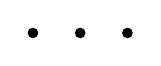
\begin{tikzpicture}[scale=0.6]
				\draw[fill] (0, 0) circle (0.1);
				\draw[fill] (1, 0) circle (0.1);
				\draw[fill] (2, 0) circle (0.1);
			\end{tikzpicture}
			}
			\hspace{3.5em}
			\centerbox{
			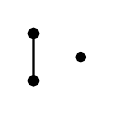
\begin{tikzpicture}[scale=0.6]
				\draw[fill, thick] (0, 0) circle (0.1) -- (0, 1) circle (0.1);
				\draw[fill] (1, 0.5) circle (0.1);
			\end{tikzpicture}
			}
			\hspace{3.5em}
			\centerbox{
			
\begin{tikzpicture}[scale=0.6]
				\draw[fill, thick] (-0.6, 1) circle (0.1) -- (0, 0) circle (0.1) -- (0.6, 1) circle (0.1);
			\end{tikzpicture}
			}
			\hspace{3.5em}
			\centerbox{
			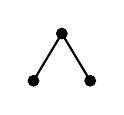
\begin{tikzpicture}[scale=0.6]
				\draw[fill, thick] (-0.6, 0) circle (0.1) -- (0, 1) circle (0.1) -- (0.6, 0) circle (0.1);
			\end{tikzpicture}
			}
			\hspace{3.5em}
			\centerbox{
			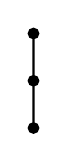
\begin{tikzpicture}[scale=0.6]
				\draw[fill, thick] (0, 0) circle (0.1) -- (0, 1) circle (0.1) -- (0, 2) circle (0.1);
			\end{tikzpicture}
			}
		\]
		Let us go through these different types of partial orders:
		\begin{description}

			\item[First type]
				All three elements are non-comparable.
				Then
				\[
					U a = \{ a \} \,, \quad
					U b = \{ b \} \,, \quad
					U c = \{ c \} \,.
				\]
				The resulting topology is the discrete topology
				\[
					\top{T}_{29} ≔ \{ ∅, \{a\}, \{b\}, \{c\}, \{a,b\}, \{a,c\}, \{b,c\}, X \} \,.
				\]

			\item[Second type]
				Precisely two elements of~$X / {∼}$ are comparable.

				Suppose first that~$\class{a} ≤ \class{b}$ and that~$\class{c}$ is not comparable to either~$\class{a}$ and~$\class{b}$.
				Then~$U a = \{ a, b \}$,~$U b = \{ b \}$,~$U c = \{ c \}$.
				The resulting topology is
				\[
					\top{T}_{27} ≔
					\{
						∅, \{ b \}, \{ c \}, \{ a, b \}, \{ b, c \}, X
					\} \,.
				\]

				By permuting the roles of~$a$,~$b$ and~$c$, we also get the topologies
				\begin{align*}
					% swap a and b
					\top{T}_{25} &≔ \{ ∅, \{ a \}, \{ c \}, \{ a, b \}, \{ a, c \}, X \} \,,
					\\
					% swap a and b
					\top{T}_{24} &≔ \{ ∅, \{ a \}, \{ b \}, \{ a, b \}, \{ b, c \}, X \} \,,
					\\
					% swap b and c
					\top{T}_{28} &≔ \{ ∅, \{ b \}, \{ c \}, \{ a, c \}, \{ b, c \}, X \} \,,
					\\
					% swap a → b → c
					\top{T}_{26} &≔ \{ ∅, \{ a \}, \{ c \}, \{ a, c \}, \{ b, c \}, X \} \,,
					\\
					% swap c → b → a
					\top{T}_{23} &≔ \{ ∅, \{ a \}, \{ b \}, \{ a, b \}, \{ a, c \}, X \} \,.
				\end{align*}

			\item[Third type]
				All elements of~$X / {∼}$ are comparable, but not linearly comparable, with a least element.

				Suppose first that~$\class{a} ≤ \class{b}, \class{c}$.
				Then~$U a = X$,~$U b = \{ b \}$,~$U c = \{ c \}$.
				The corresponding topology is
				\[
					\top{T}_{19} ≔ \{ ∅, \{ b \}, \{ c \}, \{ b, c \}, X  \} \,.
				\]

				By swapping around the roles of~$a$,~$b$ and~$c$, we also get the topologies
				\[
					\top{T}_{17} ≔ \{ ∅, \{ a \}, \{ b \}, \{ a, b \}, X  \} \,, \quad
					\top{T}_{18} ≔ \{ ∅, \{ a \}, \{ c \}, \{ a, c \}, X  \} \,.
				\]

			\item[Fourth type]
				All elements of~$X / {∼}$ are comparable, but not linearly comparable, with a greatest element.

				Suppose first that~$\class{a}, \class{b} ≤ \class{c}$.
				Then~$U a = \{ a, c \}$,~$U b = \{ b, c \}$,~$U c = \{ c \}$.
				The corresponding topology is
				\[
					\top{T}_{22} ≔ \{ ∅, \{ c \}, \{ a, c \}, \{ b, c \}, X \} \,.
				\]

				By swapping around the roles of~$a$,~$b$ and~$c$, we also get the topologies
				\[
					\top{T}_{20} ≔ \{ ∅, \{ a \}, \{ a, b \}, \{ a, c \}, X \} \,, \quad
					\top{T}_{21} ≔ \{ ∅, \{ b \}, \{ a, b \}, \{ b, c \}, X \} \,.
				\]

			\item[Fifth type]
				All elements of~$X / {∼}$ are linearly comparable.

				Suppose first that~$\class{c} ≤ \class{b} ≤ \class{a}$.
				Then~$U a = \{ a \}$,~$U b = \{ a, b \}$,~$U c = X$.
				The resulting topology is
				\[
					\top{T}_8 ≔ \{ ∅, \{ a \}, \{ a, b \}, X \} \,.
				\]

				By permuting the roles of~$a$,$~b$,~$c$, we get also the topologies
				\begin{align*}
					\top{T}_9    &≔ \{ ∅, \{ a \}, \{ a, c \}, X \} \,, \\
					\top{T}_{11} &≔ \{ ∅, \{ b \}, \{ a, b \}, X \} \,, \\
					\top{T}_{13} &≔ \{ ∅, \{ b \}, \{ b, c \}, X \} \,, \\
					\top{T}_{15} &≔ \{ ∅, \{ c \}, \{ a, c \}, X \} \,, \\
					\top{T}_{16} &≔ \{ ∅, \{ c \}, \{ b, c \}, X \} \,.
				\end{align*}

		\end{description}

	\item
		The elements~$b$ and~$c$ are equivalent, but not equivalent to~$a$.
		On the two-element quotient set~$X / {∼} = \{ \{ a \}, \{ b, c \} \}$ we have three partial orders.
		\begin{description}

			\item[First type]
				The elements of~$X / {∼}$ are not comparable.
				Then
				\[
					U a = \{ a \} \,, \quad
					U b, U c = \{ b, c \} \,.
				\]
				The resulting topology is
				\[
					\top{T}_{10} ≔ \{ ∅, \{ a \}, \{ b, c \}, X \} \,.
				\]

			\item[Second type]
				We have~$\{ a \} ≤ \{ b, c \}$.
				Then~$U a = X$ and~$U b, U c = \{ b, c \}$.
				The resulting topology is
				\[
					\top{T}_7 ≔ \{ ∅, \{ b, c \}, X \} \,.
				\]

			\item[Third type]
				We have~$\{ b, c \} ≤ \{ a \}$.
				Then~$U a = \{ a \}$ and~$U b, U c = X$.
				The resulting topology is
				\[
					\top{T}_2 ≔ \{ ∅, \{ a \}, X \}
				\]

		\end{description}

		By swapping the roles the~$a$,~$b$ and~$c$ around, we get the following additional topologies:
		\begin{gather*}
			% all permutations of { ∅, {a}, {b, c}, X }
			\top{T}_{12} ≔ \{ ∅, \{ b \}, \{ a, c \}, X \} \,, \quad
			\top{T}_{14} ≔ \{ ∅, \{ c \}, \{ a, b \}, X \} \,, \quad
			% all permutations of { ∅, {b, c}, X }
			\top{T}_5 ≔ \{ ∅, \{ a, b \}, X \} \,,
			\\
			\top{T}_6 ≔ \{ ∅, \{ a, c \}, X \} \,, \quad
			% permutations of \{ ∅, \{ a \}, X \}
			\top{T}_3 ≔ \{ ∅, \{ b \}, X \} \,, \quad
			\top{T}_4 ≔ \{ ∅, \{ c \}, X \} \,.
		\end{gather*}

	\item
		All three elements of~$X$ are equivalent.
		The quotient set~$X / {∼}$ consists of one element, whence there is precisely one partial order on it.
		The corresponding topology is given by the indiscrete topology
		\[
			\top{T}_1 ≔ \{ ∅, X \} \,.
		\]

\end{itemize*}

We have overall found~$29$ topologies on the three-element set~$X = \{ a, b, c \}$.
The inclusions between these topologies is depicted in \cref{topologies on a three element set}.
\begin{figure}
	\centering
	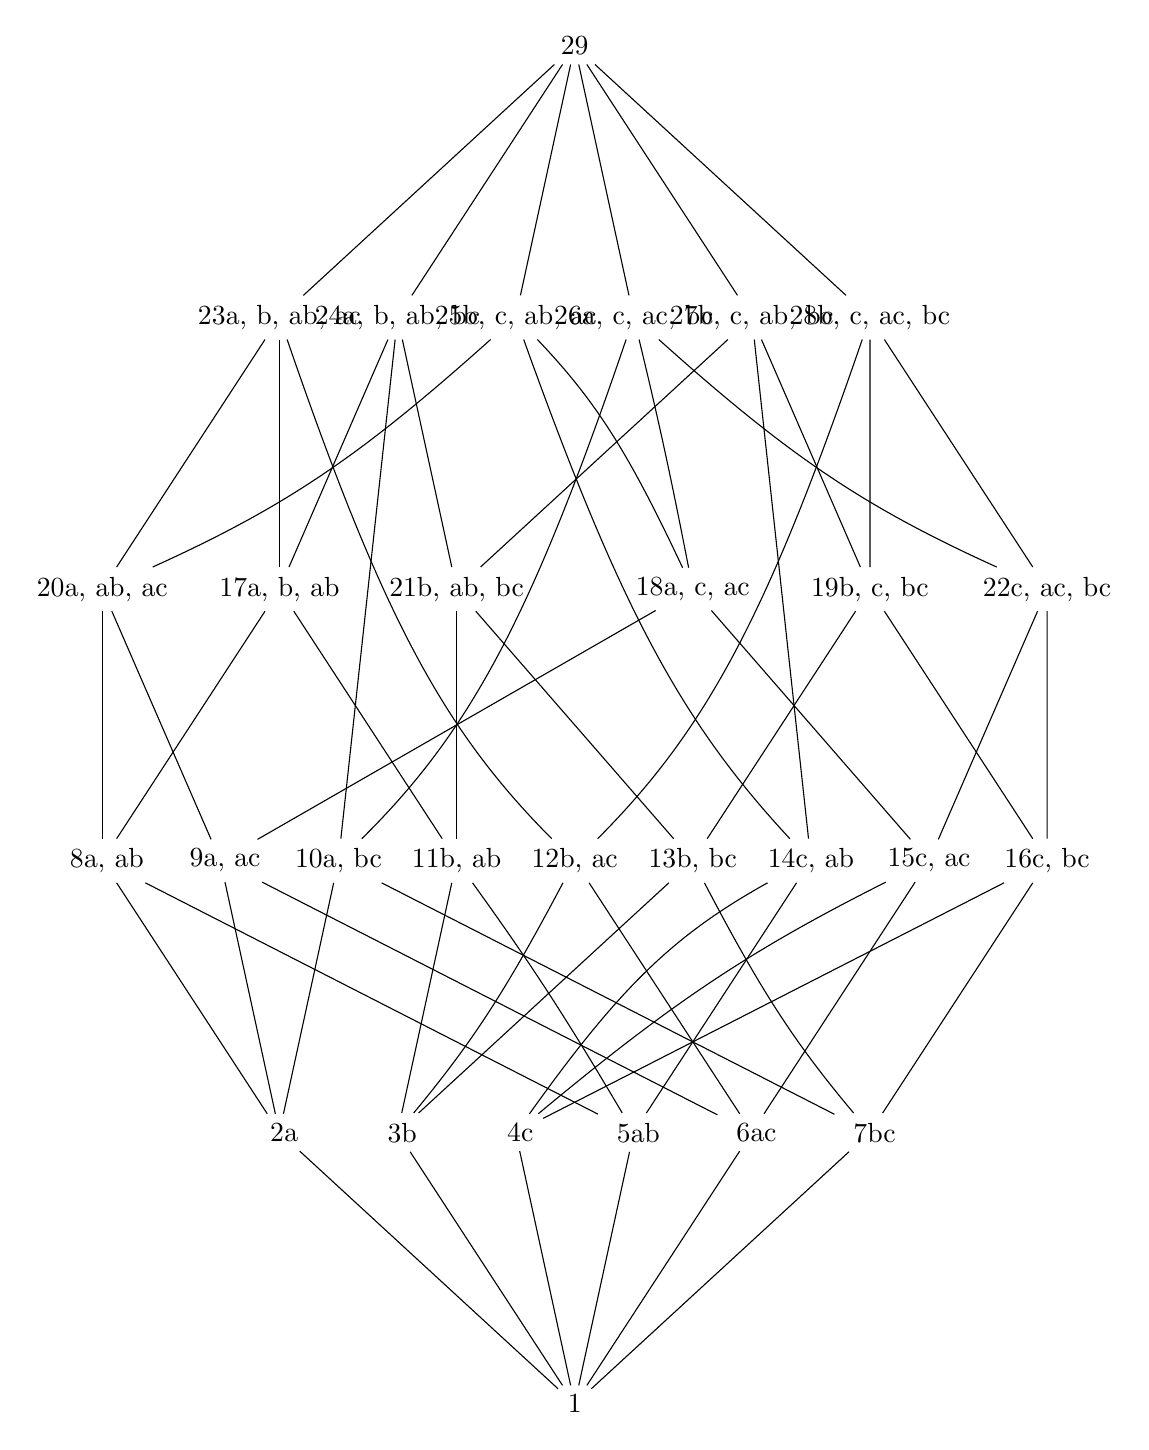
\begin{tikzpicture}[xscale = 0.75, yscale = 3.45]
		% no elements
		\node  (1) at ( 8, 0) {$1$};
		% one element
		\node  (2) at ( 3, 1) {\topel{ 2}{a}};
		\node  (3) at ( 5, 1) {\topel{ 3}{b}};
		\node  (4) at ( 7, 1) {\topel{ 4}{c}};
		\node  (5) at ( 9, 1) {\topel{ 5}{ab}};
		\node  (6) at (11, 1) {\topel{ 6}{ac}};
		\node  (7) at (13, 1) {\topel{ 7}{bc}};
		% two elements
		\node  (8) at ( 0, 2) {\topel{ 8}{a, ab}};
		\node  (9) at ( 2, 2) {\topel{ 9}{a, ac}};
		\node (10) at ( 4, 2) {\topel{10}{a, bc}};
		\node (11) at ( 6, 2) {\topel{11}{b, ab}};
		\node (12) at ( 8, 2) {\topel{12}{b, ac}};
		\node (13) at (10, 2) {\topel{13}{b, bc}};
		\node (14) at (12, 2) {\topel{14}{c, ab}};
		\node (15) at (14, 2) {\topel{15}{c, ac}};
		\node (16) at (16, 2) {\topel{16}{c, bc}};
		% three elements
		\node (20) at ( 0, 3) {\topel{20}{a, ab, ac}};
		\node (17) at ( 3, 3) {\topel{17}{a, b, ab}};
		\node (21) at ( 6, 3) {\topel{21}{b, ab, bc}};
		\node (18) at (10, 3) {\topel{18}{a, c, ac}};
		\node (19) at (13, 3) {\topel{19}{b, c, bc}};
		\node (22) at (16, 3) {\topel{22}{c, ac, bc}};
		% four elements
		\node (23) at ( 3, 4) {\topel{23}{a, b, ab, ac}};
		\node (24) at ( 5, 4) {\topel{24}{a, b, ab, bc}};
		\node (25) at ( 7, 4) {\topel{25}{b, c, ab, ac}};
		\node (26) at ( 9, 4) {\topel{26}{a, c, ac, bc}};
		\node (27) at (11, 4) {\topel{27}{b, c, ab, bc}};
		\node (28) at (13, 4) {\topel{28}{b, c, ac, bc}};
		% six elements
		\node (29) at ( 8, 5) {$29$};
		% arrows from no elements to one element;
		\draw  (1) --  (2);
		\draw  (1) --  (3);
		\draw  (1) --  (4);
		\draw  (1) --  (5);
		\draw  (1) --  (6);
		\draw  (1) --  (7);
		% arrows from one elements to two elements
		\draw  (2) --  (8);
		\draw  (2) --  (9);
		\draw  (2) -- (10);
		\draw  (3) -- (11);
		\draw  (3) to[bend right = 3.8] (12);
		\draw  (3) -- (13);
		\draw  (4) to[bend left  = 5] (14);
		\draw  (4) to[bend left  = 2] (15);
		\draw  (4) -- (16);
		\draw  (5) --  (8);
		\draw  (5) to[bend right = 1.7] (11);
		\draw  (5) -- (14);
		\draw  (6) --  (9);
		\draw  (6) -- (12);
		\draw  (6) -- (15);
		\draw  (7) -- (10);
		\draw  (7) to[bend left  = 4] (13);
		\draw  (7) -- (16);
		% arrows from two elements to three elements
		\draw  (8) -- (17);
		\draw  (8) -- (20);
		\draw  (9) -- (18);
		\draw  (9) -- (20);
		\draw (11) -- (17);
		\draw (11) -- (21);
		\draw (13) -- (19);
		\draw (13) -- (21);
		\draw (15) -- (18);
		\draw (15) -- (22);
		\draw (16) -- (19);
		\draw (16) -- (22);
		% arrows from two elements to four elements
		\draw (10) -- (24);
		\draw (10) to[bend right = 10.2] (26);
		\draw (12) to[bend left  = 10] (23);
		\draw (12) to[bend right = 10] (28);
		\draw (14) to[bend left  = 9] (25);
		\draw (14) -- (27);
		% arrows from three elements to four elements
		\draw (17) -- (23);
		\draw (17) -- (24);
		\draw (18) to[bend right = 6] (25);
		\draw (18) to[bend right = 3] (26);
		\draw (19) -- (27);
		\draw (19) -- (28);
		\draw (20) -- (23);
		\draw (20) to[bend right = 2.7] (25);
		\draw (21) -- (24);
		\draw (21) -- (27);
		\draw (22) to[bend left  = 2.7] (26);
		\draw (22) -- (28);
		% arrows from four elements to six elements
		\draw (23) -- (29);
		\draw (24) -- (29);
		\draw (25) -- (29);
		\draw (26) -- (29);
		\draw (27) -- (29);
		\draw (28) -- (29);
	\end{tikzpicture}
	\caption{The topologies on~$\{ a, b, c \}$.}
	\label{topologies on a three element set}
\end{figure}

\subsection{Exercise~1.2}

\begin{lemma}
	\label{comparison of subbases}
	Let~$X$ be a set and let~$\subbasis{S}_1$ and~$\subbasis{S}_2$ be two collections of subsets of~$X$.
	Suppose that for every~$S_2 ∈ \basis{S}_2$ and every~$x ∈ S_2$ there exists some~$S_1 ∈ \basis{S}_1$ such that~$x ∈ S_1$ and~$S_1 ⊆ S_2$.
	Then the topology generated by~$\basis{S}_1$ is finer than the topology generated by~$\basis{S}_2$.
\end{lemma}

\begin{proof}
	Let~$\top{T}_1$ and~$\top{T}_2$ be the topologies on~$X$ generated by~$\subbasis{S}_1$ and~$\subbasis{S}_2$ respectively.
	Every set belonging to~$\subbasis{S}_1$ is contained in~$\top{T}_1$, and the given assumption tells us that every set belonging to~$\subbasis{S}_2$ is a union of sets belonging to~$\subbasis{S}_1$.
	Hence, every set belonging to~$\subbasis{S}_2$ also belongs to~$\top{T}_1$.
	Consequently,~$\top{T}_2$ is a subset of~$\top{T}_1$.
\end{proof}

\begin{proposition}
	\label{induced basis for product topology}
	Let~$(X_α)_{α ∈ A}$ be a family of topological spaces, and for every index~$α ∈ A$ let~$\basis{B}_α$ be a basis of~$X_α$.
	Let~$\basis{B}$ be the collection of all subsets of~$∏_{α ∈ A} X_α$ of the form~$∏_{α ∈ A} U_α$ for which there exists a finite subset~$A'$ of~$A$ such that~$U_α ∈ \basis{B}_α$ for every~$α ∈ A'$ and~$U_α = X_α$ whenever~$α ∉ A'$.
	The set~$\basis{B}$ is a basis for~$∏_{α ∈ A} X_α$.
\end{proposition}

\begin{proof}
	Given finitely many distinct indices~$α_1, \dotsc, α_n ∈ A$ and a subset~$S_i$ of~$X_{α_i}$ for every~$i = 1, \dotsc, n$, we denote by~$P(S_1, \dotsc, S_n)$ the subset~$∏_{α ∈ A} T_α$ of~$∏_{α ∈ A} X_α$ given by~$T_{α_i} = S_i$ for every~$i = 1, \dotsc, n$ and~$T_α = X_α$ otherwise.
	The set~$\basis{B}$ is thus given by
	\[
		\basis{B}
		≔
		\{
			P(B_1, \dotsc, B_n)
			\suchthat
			\text{$n ≥ 0$, distinct~$α_1, \dotsc, α_n ∈ A$, sets~$B_i ∈ \basis{B}_{α_i}$}
		\} \,.
	\]

	We know from Definition~1.4 that the (product) topology of~$∏_{α ∈ A} X_α$ has the collection of subsets
	\[
		\basis{B}_Π
		≔
		\{
			P(U_1, \dotsc, U_n)
			\suchthat
			\text{$n ≥ 0$, $α_1, \dotsc, α_n ∈ A$ distinct, $U_i ⊆ X_{α_i}$ open}
		\}
	\]
	as a basis.
	The sets belonging to~$\basis{B}_α$ are open in~$X_α$, whence~$\basis{B}$ is a subset of~$\basis{B}_Π$.
	Consequently, the topology generated by~$\basis{B}$ is coarser than the product topology.

	Let~$U$ be an element of~$\basis{B}_Π$ and let~$x$ be a point in~$I$.
	The set~$U$ is of the form~$P(U_1, \dotsc, U_n)$ for distinct indices~$α_1, \dotsc, α_n ∈ A$ and open subsets~$U_i$ of~$X_{α_i}$.
	That~$x = (x_α)_α$ is in~$U$ means that~$x_{α_i} ∈ U_i$ for every~$i = 1, \dotsc, n$.
	Since each set~$\basis{B}_α$ is a basis for the respective topological space~$X_α$, there exists for every~$i = 1, \dotsc, n$ some set~$B_i$ belonging to~$\basis{B}_{α_i}$ such that~$x_i ∈ B_i$ and~$B_i ⊆ U_i$.
	It follows that the set~$B ≔ P(B_1, \dotsc, B_n)$, which belongs to~$\basis{B}$, satisfies~$x ∈ B$ and~$B ⊆ U$.

	This shows, according to \cref{comparison of subbases}, that the topology generated by~$\basis{B}$ is finer than the product topology.
\end{proof}

We observe that we have for every point~$y$ in~$\ball_n(x, ε)$ the inequalities
\[
	\abs{x_i - y_i}
	≤
	\sqrt{ (x_1 - y_1)^2 + \dotsb + (x_n - y_n)^2 }
	=
	\norm{x - y}
	<
	ε \,.
\]
Consequently, we have
\[
	\ball_n(x, ε) ⊆ \ball_1(x_1, ε) × \dotsb × \ball_1(x_n, ε) \,.
\]
Conversely, we have every point~$y$ in~$\ball_1(x_1, ε_1) × \dotsb × \ball_n(x_n, ε_n)$ for the radius~$ε ≔ \max(ε_1, \dotsc, ε_n)$ the inequalities
\[
	\norm{x - y}
	=
	\sqrt{ \abs{x_1 - y_1}^2 + \dotsb + \abs{x_n - y_n}^2 }
	<
	\sqrt{ ε_1^2 + \dotsb + ε_n^2 }
	≤
	\sqrt{ n ε^2 }
	=
	\sqrt{n} ε \,.
\]
Consequently, we have
\[
	\ball_1(x_1, ε_1) × \dotsb × \ball_1(x_1, ε_1) ⊆ \ball_n(x, \sqrt{n} ε) \,.
\]

A basis for the topology on~$ℝ^n$ is given by
\[
	\basis{B}_n ≔ \{ \ball_n(x, ε) \suchthat x ∈ ℝ^n, ε > 0 \} \,.
\]
It follows from \cref{induced basis for product topology} that a basis for the product topology on~$ℝ^n$ (when~$ℝ^n$ is viewed as the iterated product~$ℝ × \dotsb × ℝ$) is given by
\begin{align*}
	\basis{B}^n
	&≔
	\{ B_1 × \dotsb × B_n \suchthat B_i ∈ \basis{B}_1 \} \\
	&=
	\{
		\ball_1(x_1, ε_1) × \dotsb × \ball_1(x_n, ε_n)
		\suchthat
		x_1, \dotsc, x_n ∈ ℝ,
		ε_1, \dotsc, ε_n > 0
	\} \,.
\end{align*}
We will use \cref{comparison of subbases} to show that~$\basis{B}^n$ and~$\basis{B}_n$ generate the same topology.

Let~$y$ be a point is some open ball~$\ball_n(x, ε)$.
It follows that there exists some radius~$δ > 0$ with~$\ball_n(y, δ) ⊆ \ball_n(x, ε)$ (one may choose~$δ$ as~$ε - \norm{x - y}$).
It follows for the set~$U ≔ \ball_1(y_1, δ / \sqrt{n}) × \dotsb × \ball_1(y_n, δ / \sqrt{n})$, which belongs to~$\basis{B}^n$, that~$y ∈ U$ and~$U ⊆ \ball_n(y, δ) ⊆ \ball_n(x, ε)$.
According to \cref{comparison of subbases}, this shows that the topology generated by~$\basis{B}^n$ is finer than the topology generated by~$\basis{B}_n$.

Let~$y$ be a point in the set~$W ≔ \ball_1(x_1, ε_1) × \dotsb × \ball_1(x_n, ε_n)$.
This means that~$y_i ∈ \ball_1(x_i, ε_i)$ for every~$i = 1, \dotsc, n$.
There hence exists for every~$i = 1, \dotsc, n$ some radius~$δ_i > 0$ with~$\ball_1(y_i, δ_i) ⊆ \ball(x_i, ε_i)$.
It follows for~$δ ≔ \min(δ_1, \dotsc, δ_n)$ and the set~$V ≔ \ball(y_1, δ) × \dotsb × \ball(y_n, δ)$ that~$V ⊆ W$.
It further follows for the set~$U ≔ \ball_n(y, δ)$, which belongs to~$\basis{B}^n$, that~$y ∈ U$ and~$U ⊆ V ⊆ W$.
According to \cref{comparison of subbases}, this shows that the topology generated by~$\basis{B}_n$ is finer than the topology generated by~$\basis{B}^n$.

